\section{Design}
\label{sec:design}

O design do protótipo foi concebido a partir das definições oriundas da matriz morfológica e também de inspirações de ROVs comerciais, como o \textit{Seafox} e o \textit{BlueROV2}, mostrados na Figura \ref{fig:seafoxbluerov2}.

\begin{figure}[h]
	\centering
	\caption[ROVs que inspiraram o design do BROV]{ROVs que inspiraram o design do BROV: \textit{Seafox} (à esquerda) e \textit{BlueROV2} (à direita)}
	\label{fig:seafoxbluerov2}
	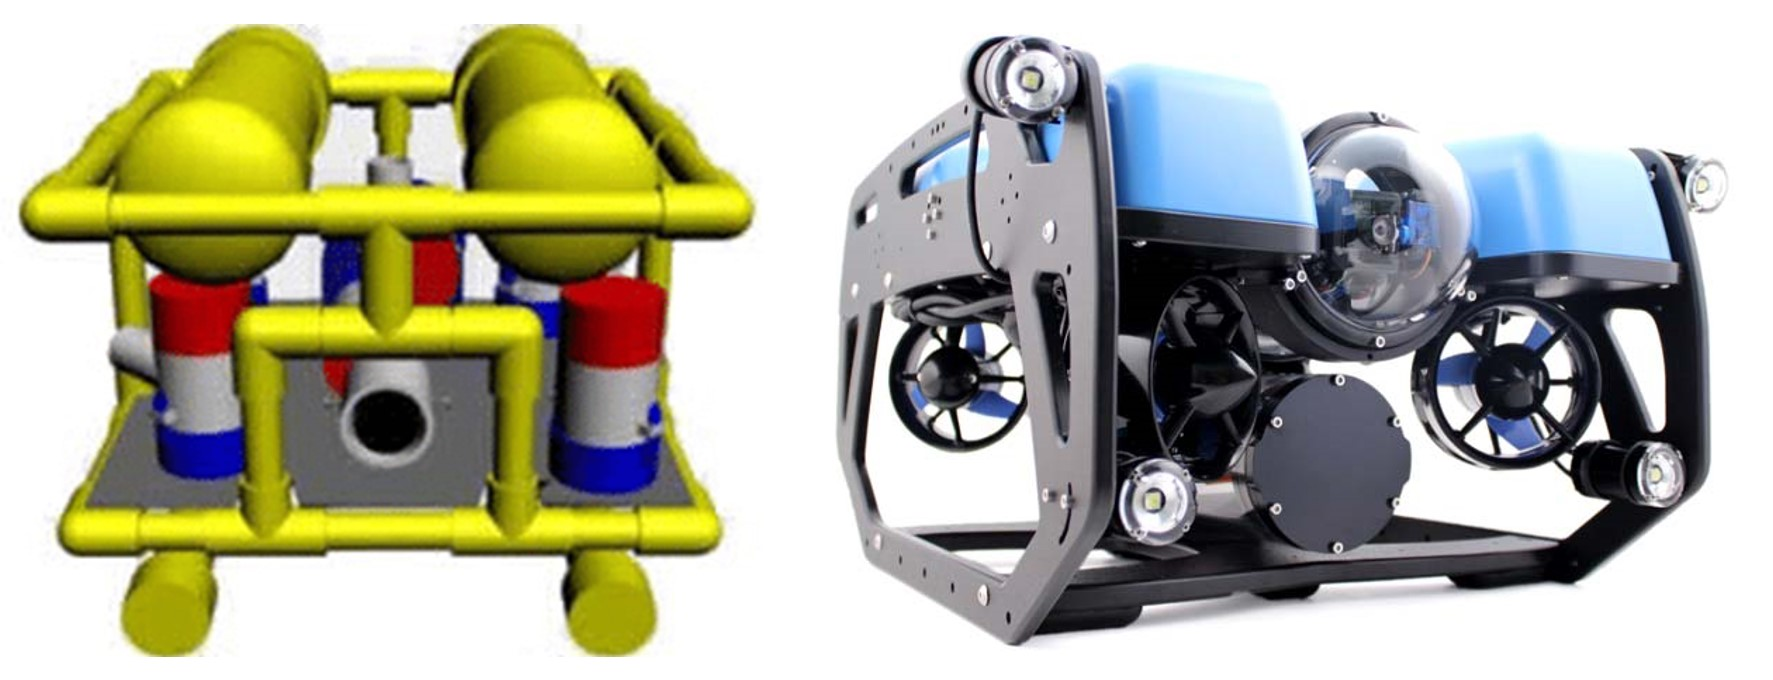
\includegraphics[width=0.8\linewidth]{images/seafox_bluerov2}\\
	\footnotesize Fonte: \cite{Rocha2014} e \cite{bluerov2}
	
\end{figure}

Para escolha do material da estrutura do BROV foram levados em consideração o baixo custo e a versatilidade para futuras integrações de novos sensores. Dessa forma, optou-se por utilizar estrutura tubular, como a do \textit{Seafox}. O design conceitual da estrutura está mostrado na Figura \ref{fig:brov-frame}.

\begin{figure}[h]
	\centering
	\caption{Estrutura conceitual do BROV}
	\label{fig:brov-frame}
	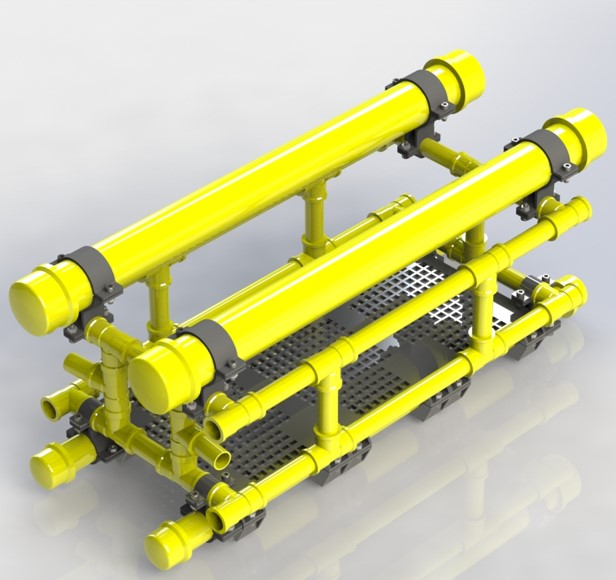
\includegraphics[width=0.7\linewidth]{images/brov-frame}\\
	\footnotesize Fonte: Autores
\end{figure}

Para a fixação da estrutura tubular entre si foram utilizados conectores do tipo ``tê soldável'' e ``joelho 90°'', itens comerciais retirados do catálogo da Tigre\,\textsuperscript{\tiny\textregistered} \cite{Tigre2009}. Nos casos em que não foi possível a união tubular através desses conectores, optou-se por utilizar peças impressas 3D em ABS, modeladas exclusivamente para esse fim, evitando-se uso de abraçadeiras metálicas e do tipo ``enforca-gato'', que viriam a prejudicar a estética do ROV. Julgou-se necessário também a utilização de uma base (impressa 3D) para apoio e fixação dos mais diversos tipos de componentes, como \textit{housings}, fios e acessórios. Parafusos e porcas de aço inoxidável austenítico 304 foram selecionados como elementos padrão de fixação. 

No design do ROV também foi levado em consideração a versatilidade no controle da flutuabilidade. Os dois maiores tubos da parte superior podem acomodar um grande volume de espuma expansível, que possui baixa densidade, da ordem de 0,1 g/cm³. Caso os tubos não resistam aos esforços de pressão na profundidade especificada pelo projeto, a espuma poderá ser aplicada para evitar o colapso do tubo, ao mesmo tempo que favorecerá o empuxo se comparado com o preenchimento com água. De modo análogo, os tubos inferiores foram pensados para um eventual acréscimo discreto de massa -- com bolas de gude, por exemplo -- para ajuste da altura do centro de gravidade do protótipo. Os tubos menores, que compõem a parte central da estrutura, foram mantidos abertos para circulação de água.

O sistema de propulsão foi fortemente inspirado no \textit{BlueROV2}, que é um ROV \textit{open source} da empresa \textit{BlueRobotics}. Algumas alterações em nível de escala, elementos de fixação e componentes do duto canalizador foram feitas em relação aos presentes no \textit{BlueROV2}, de modo a tornar a montagem compatível com o motor \textit{brushless} A2212, que será utilizado no projeto. A Figura \ref{fig:propulsor} mostra o propulsor que será utilizado no BROV.

\begin{figure}[h]
	\centering
	\caption{Propulsor do BROV}
	\label{fig:propulsor}
	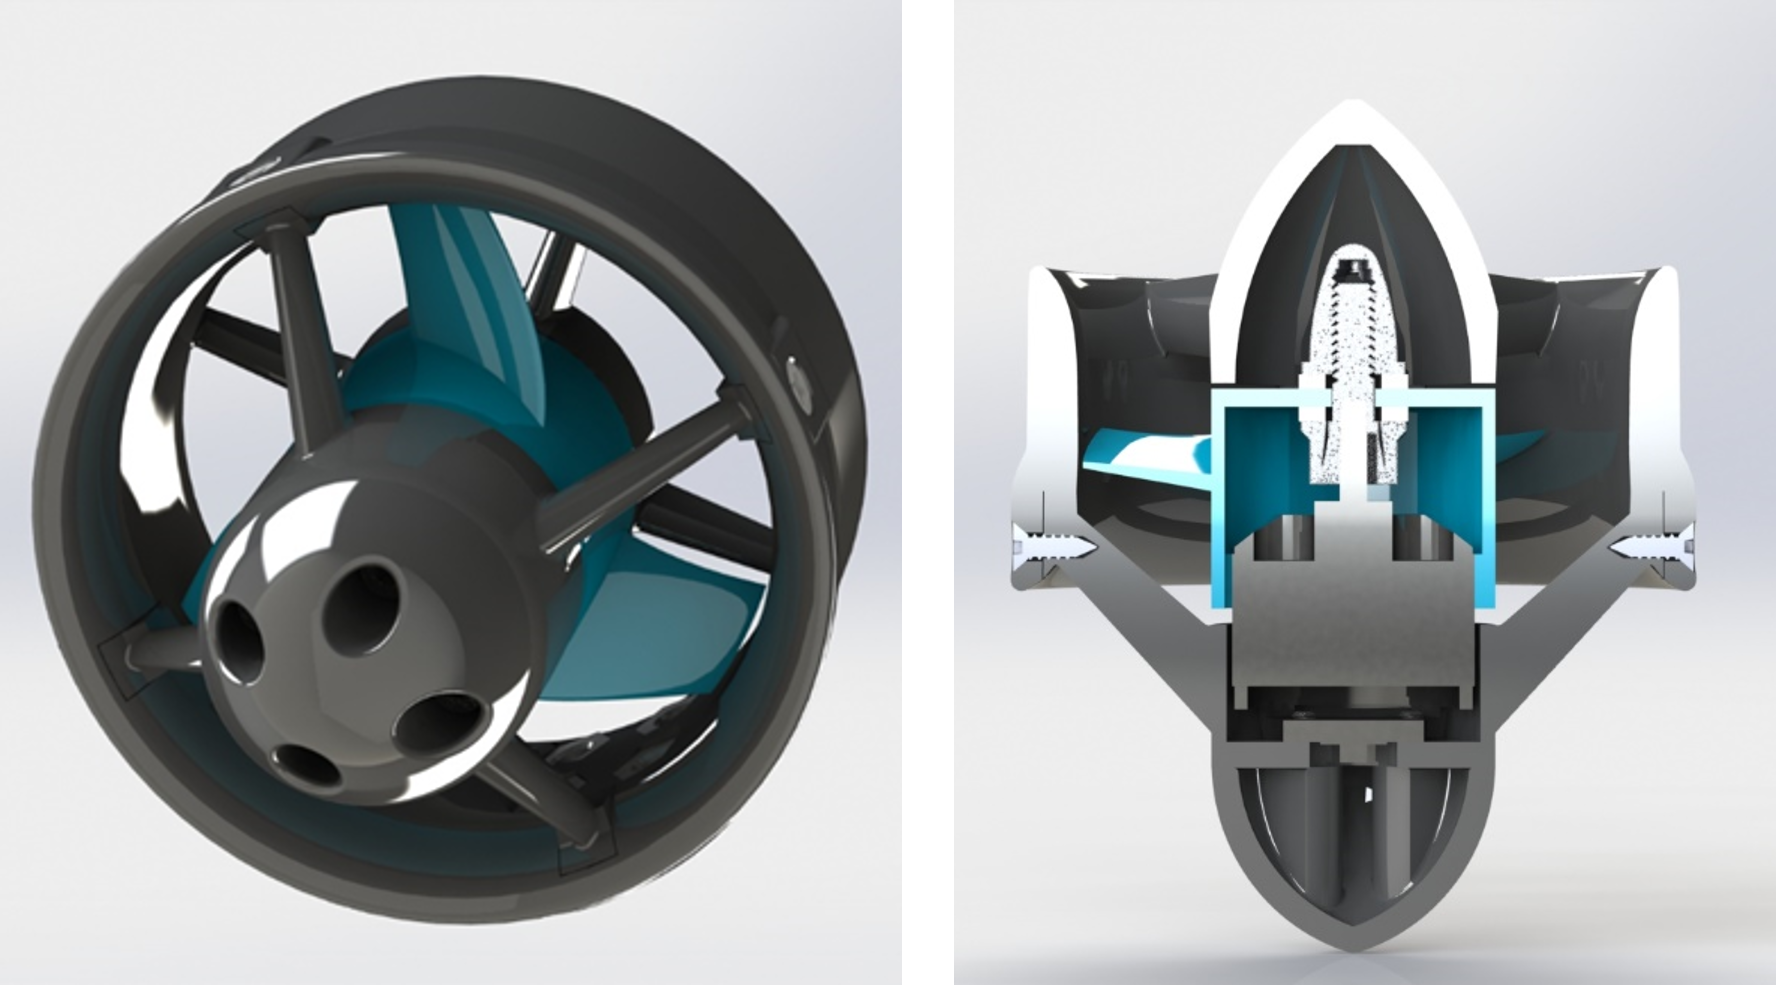
\includegraphics[width=0.8\linewidth]{images/propulsor}\\
	\footnotesize Fonte: Autores
\end{figure}

Os motivos pela escolha desse modelo de motor foram: não necessidade de selagem, facilidade de montagem, alto torque e baixo \textit{lead time}. A alocação dos \textit{thrusters} -- mostrada na Figura \ref{fig:posicionamento-thrusters} -- foi pensada de modo a de obter o controle dos 3 graus de liberdade translacionais -- \textit{surge}, \textit{sway} e \textit{heave}  -- e de 2 rotacionais  -- \textit{roll} e \textit{yaw} \cite{Antonelli2018}.

\begin{figure}[h]
	\centering
	\caption{Posicionamento dos thrusters}
	\label{fig:posicionamento-thrusters}
	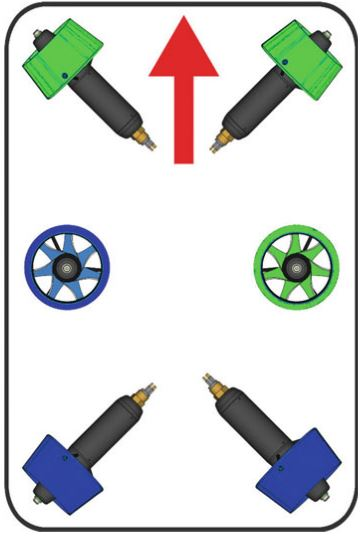
\includegraphics[width=0.25\linewidth]{images/alocacao-motores}\\
	\footnotesize Fonte: \cite{Antonelli2018}
\end{figure}


No momento em que foi escrito esse relatório o propulsor se encontrava em fase de testes, tendo a hélice e demais acessórios sido fabricados em ABS, em uma impressora 3D, conforme indicado pela Figura \ref{fig:prototipacao}. A próxima etapa a ser realizada para modelagem computacional do sistema de propulsão consiste no levantamento da curva Corrente x Torque do motor através de testes em um aquário adquirido pela equipe, conforme indicado pela Figura \ref{fig:aquario}, de modo que seja possível estimar o comportamento dinâmico do ROV quando submerso. 

\begin{figure}[h]
	\centering
	\caption{Prototipação do propulsor}
	\label{fig:prototipacao}
	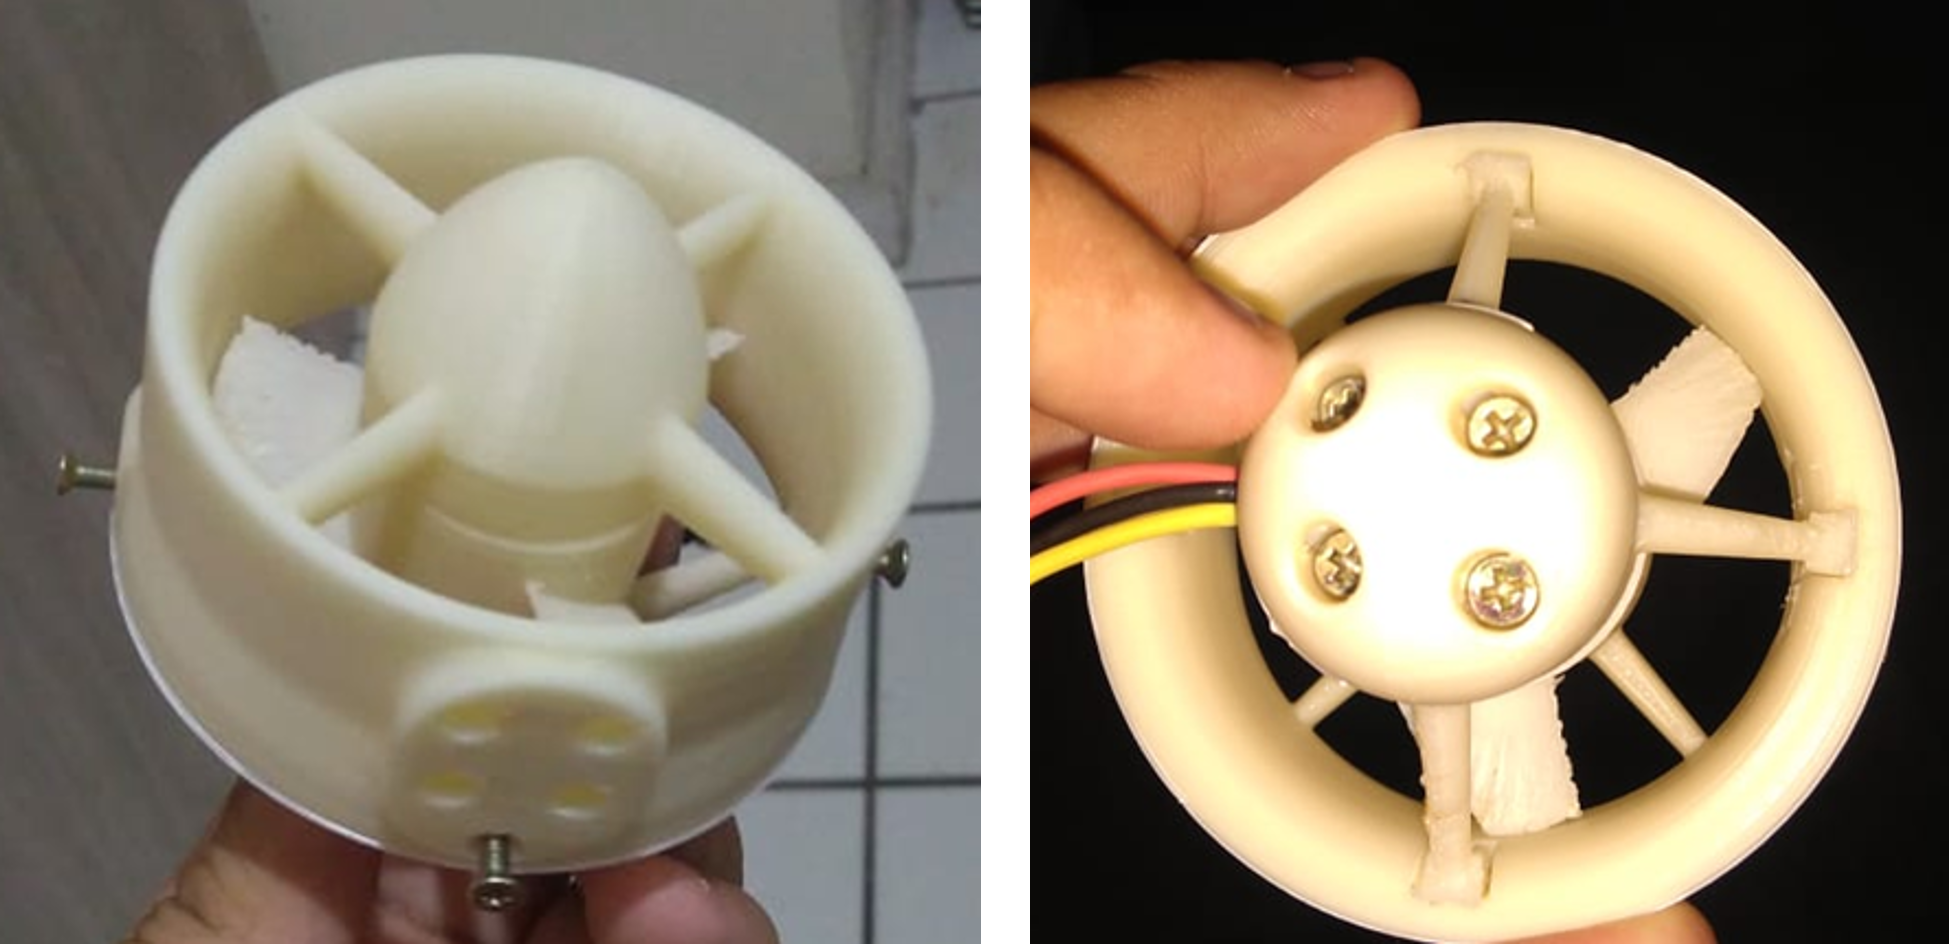
\includegraphics[width=0.8\linewidth]{images/prototipacao}\\
	\footnotesize Fonte: Autores
\end{figure}


\begin{figure}[h]
	\centering
	\caption{Aquário para testes de propulsão e comunicação}
	\label{fig:aquario}
	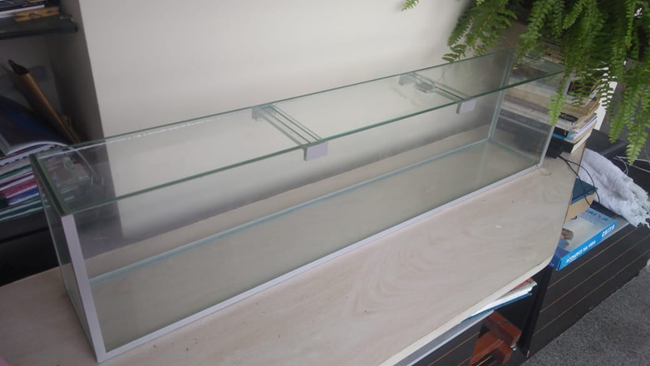
\includegraphics[width=0.8\linewidth]{images/aquario}\\
	\footnotesize Fonte: Autores
\end{figure}

\textit{Housings} tiveram que ser projetadas para uma vedação confiável da câmera monocular juntamente com seu controlador, assim como dos componentes eletrônicos de controle -- Arduíno, IMU e bateria. 

O corpo da \textit{housing} da câmera foi concebido para ser impresso 3D, com um visor de policarbonato na parte frontal, comprimido com parafusos e vedado com \textit{o-ring}. A fixação na estrutura se dará por meio do uso de abraçadeiras metálicas, de modo que seja permitida a sua rápida montagem e desmontagem, sem que haja nenhum tipo de perfuração. A Figura \ref{fig:housing-camera} mostra o projeto conceitual dessa \textit{housing}. A outra \textit{housing}, que acomodará os demais componentes eletrônicos e bateria, ainda está em desenvolvimento.

\begin{figure}[h]
	\centering
	\caption{Projeto conceitual da \textit{housing} da câmera e seu controlador}
	\label{fig:housing-camera}
	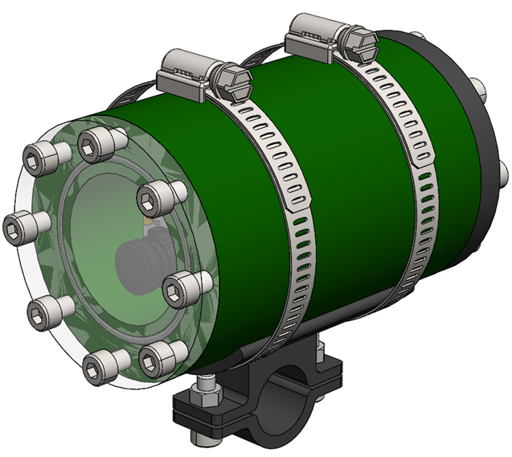
\includegraphics[width=0.5\linewidth]{images/housing-camera}\\
	\footnotesize Fonte: Autores
\end{figure}


Para prover iluminação na profundidade de 10 m, a equipe optou por utilizar uma solução de mercado já pronta: uma lanterna de pesca à prova d'água de baixo custo com fonte de alimentação própria, mostrada na Figura \ref{fig:lanterna}.

\begin{figure}[h]
	\centering
	\caption{Lanterna que será usada no BROV}
	\label{fig:lanterna}
	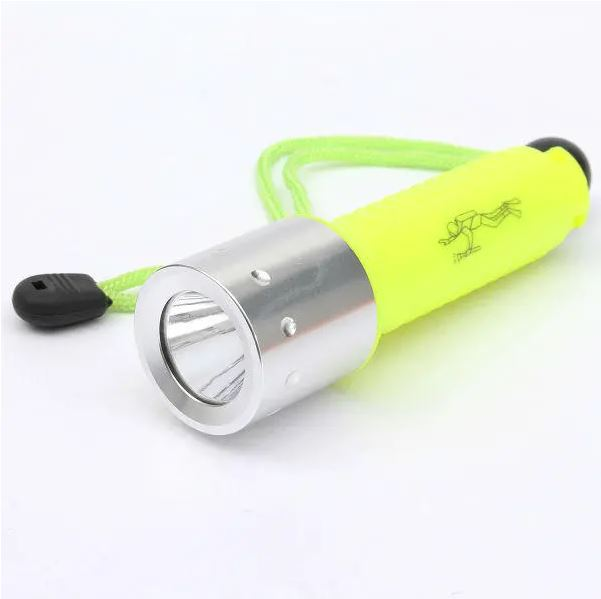
\includegraphics[width=0.4\linewidth]{images/lanterna}\\
	\footnotesize Fonte: \href{https://www.banggood.com/pt/Wholesale-Upgrade-2-T6-1600LM-3-Modes-Waterproof-LED-Flashlight-p-54536.html?imageAb=2&utm_campaign=3820755_54536&utm_content=3853&p=0101161305742201503R&cur_warehouse=CN&akmClientCountry=BR}{Banggod}
\end{figure}

Além dos componentes mencionados acima, também serão acomodados no BROV sensores de ultrassom para mapeamento e comunicação. Todos esses itens estão representados nas vistas de montagem das Figuras \ref{fig:vista-isometrica}, \ref{fig:vista-frontal}, \ref{fig:vista-lateral} e \ref{fig:vista-superior}.

\begin{figure}[h!]
	\centering
	\caption{Vista isométrica do BROV conceitual}
	\label{fig:vista-isometrica}
	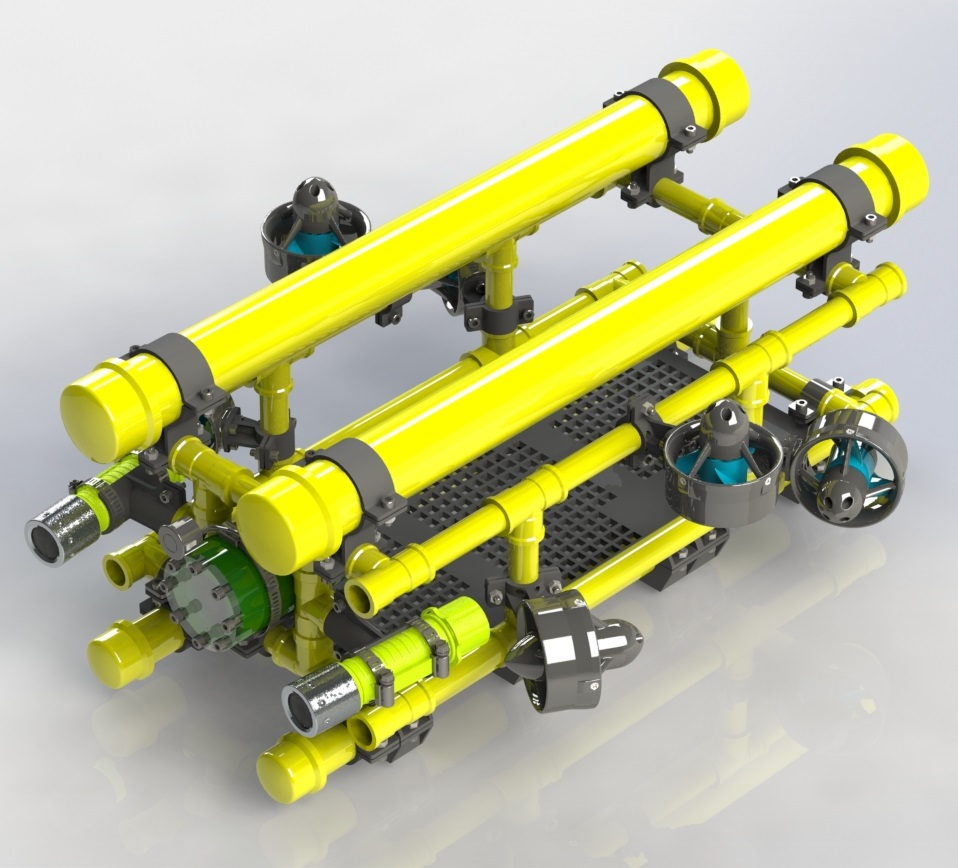
\includegraphics[width=0.7\linewidth]{images/vista-isometrica-cut}\\
	\footnotesize Fonte: Autores
\end{figure}

\begin{figure}[h!]
	\centering
	\caption{Vista frontal do BROV conceitual}
	\label{fig:vista-frontal}
	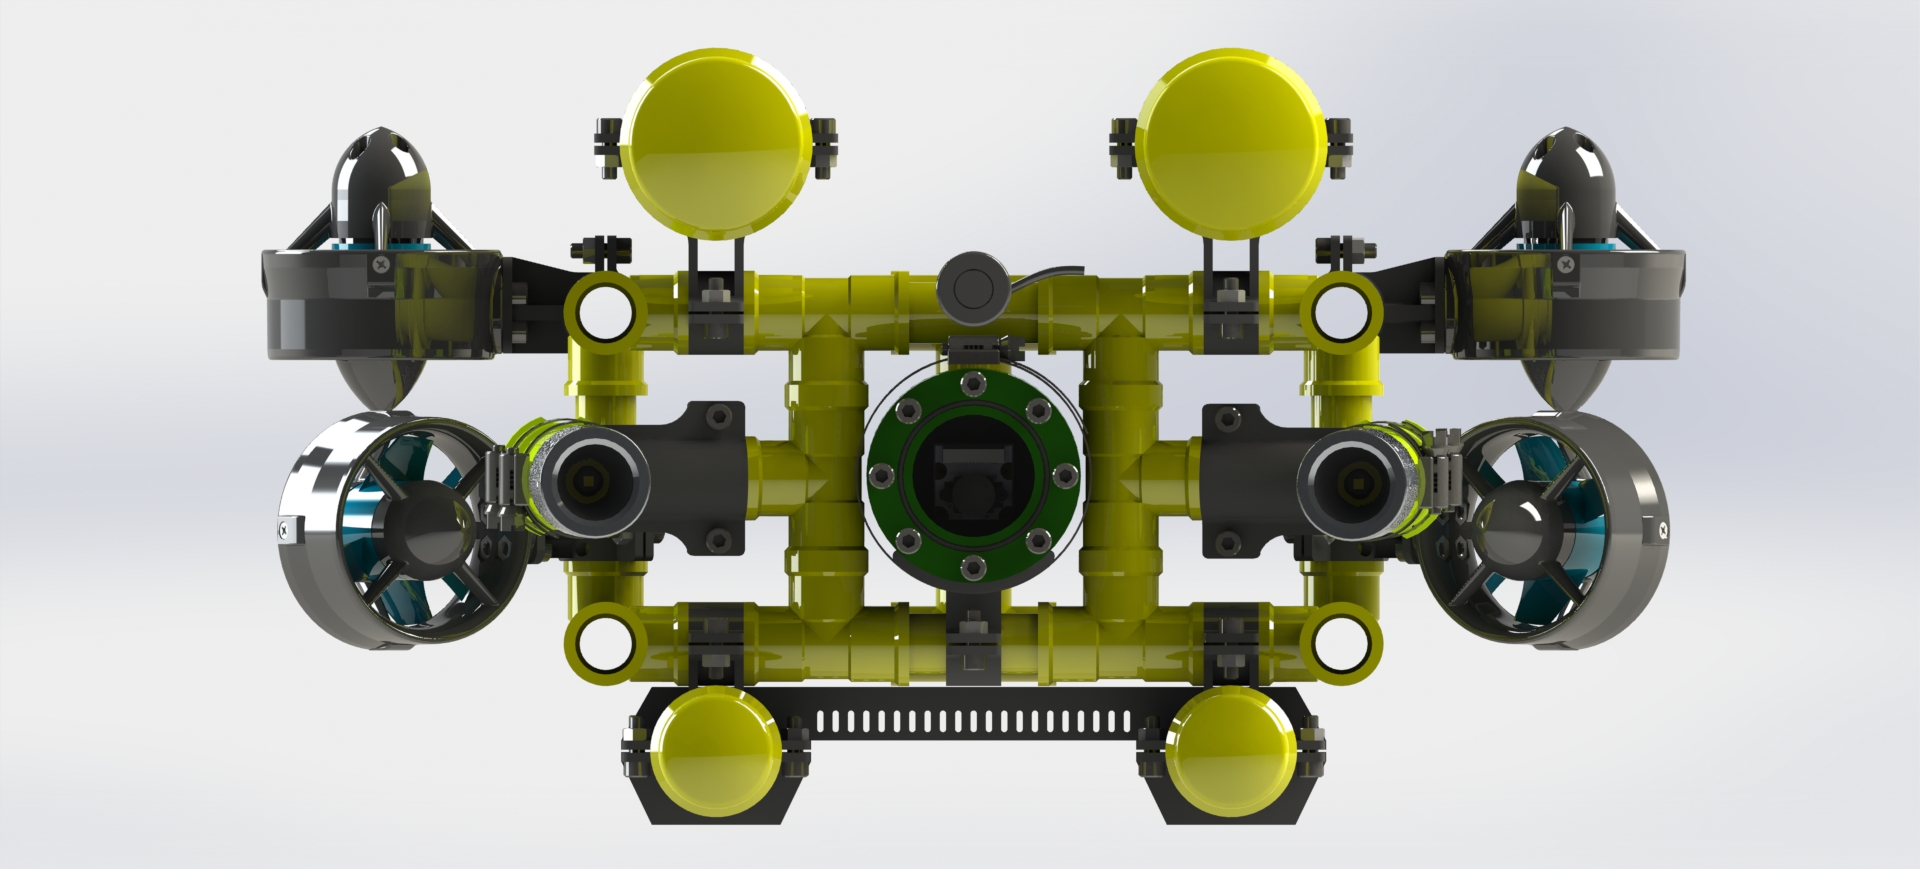
\includegraphics[width=0.7\linewidth]{images/vista-frontal}\\
	\footnotesize Fonte: Autores
\end{figure}

\begin{figure}[h!]
	\centering
	\caption{Vista lateral do BROV conceitual}
	\label{fig:vista-lateral}
	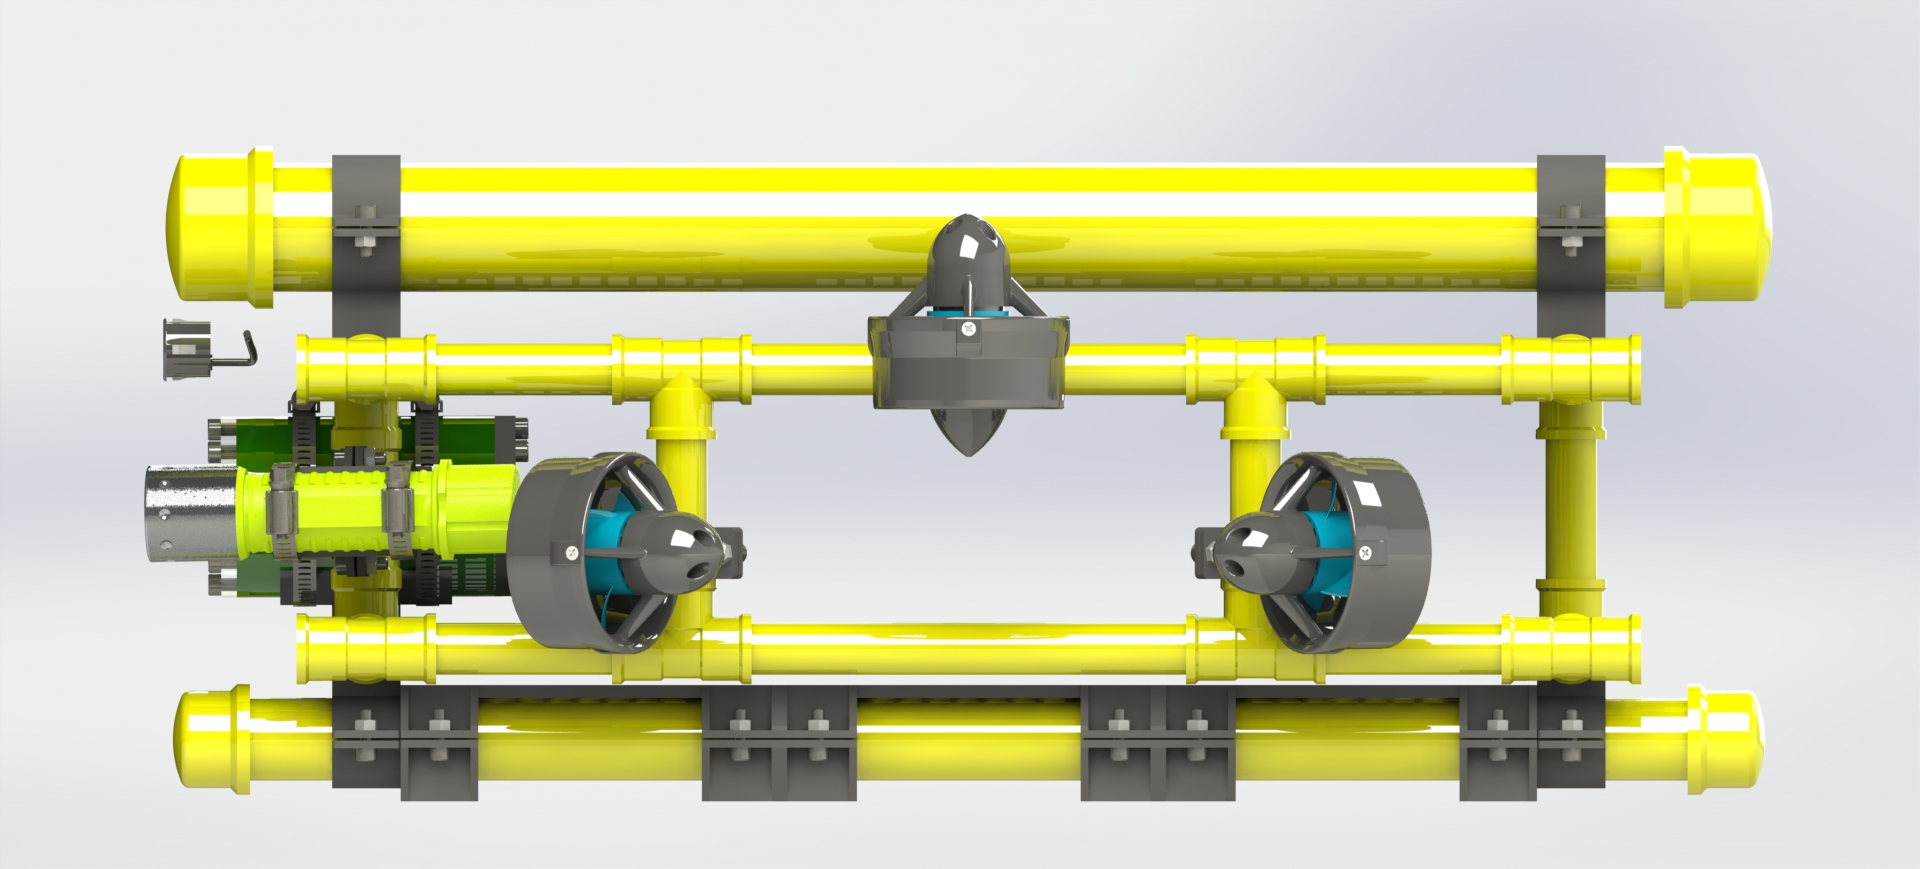
\includegraphics[width=0.7\linewidth]{images/vista-lateral}\\
	\footnotesize Fonte: Autores
\end{figure}

\begin{figure}[h!]
	\centering
	\caption{Vista superior do BROV conceitual}
	\label{fig:vista-superior}
	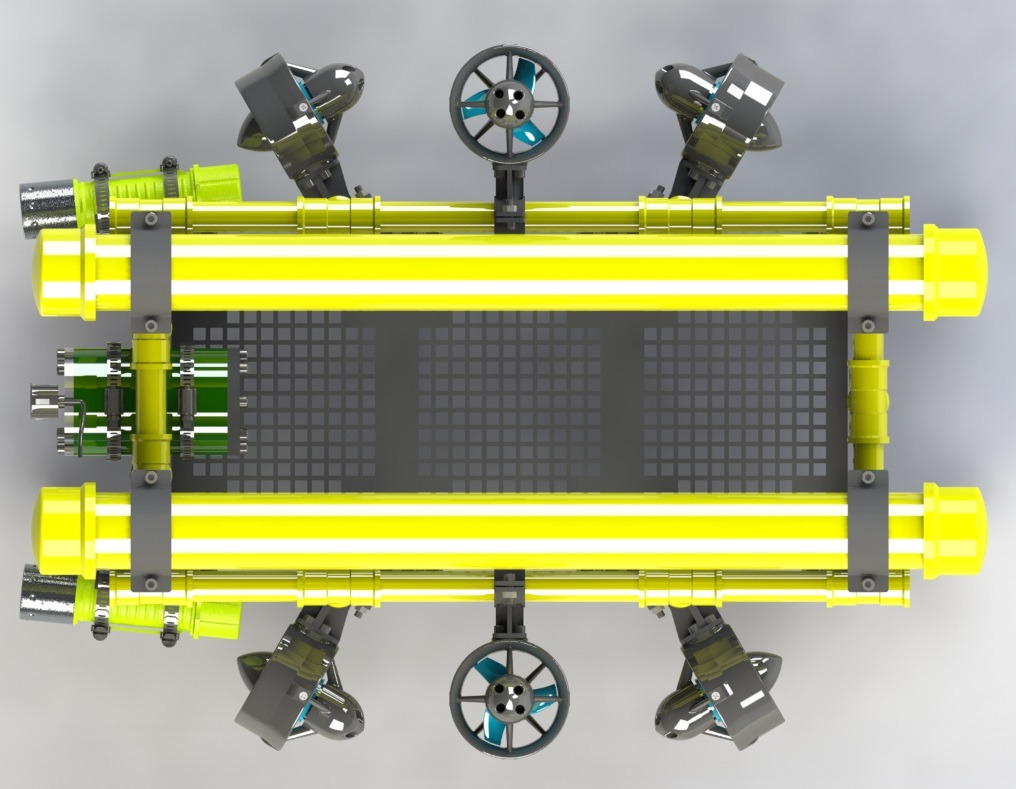
\includegraphics[width=0.7\linewidth]{images/vista-superior-cut}\\
	\footnotesize Fonte: Autores
\end{figure}
